\documentclass[11pt,a4paper]{article}
\usepackage[english]{babel}
\renewcommand{\tablename}{Tabla}
\renewcommand{\figurename}{Figura}
\usepackage{amsmath,amssymb}
\usepackage{geometry}
\geometry{top=2.0cm, bottom=2.0cm, left=2.0cm, right=2.0cm}
\usepackage{booktabs}
\usepackage{graphicx}
\usepackage{xcolor}
\usepackage{hyperref}
\usepackage{microtype}
\usepackage{caption}

\definecolor{fpuna}{RGB}{0,51,102}
\hypersetup{colorlinks=true, linkcolor=fpuna, citecolor=fpuna, urlcolor=fpuna}

\title{\textbf{\Large Propuesta de Contribución Original de Tesis de Grado:}\\
\textbf{\huge DynaTex: Marco de Fusión Dinámica Heterogénea e Inferencia Adaptativa para Clasificación de Texturas}}
\author{\textbf{Tesistas:} Joaquín Delgado, Carlos Ayala \quad \textbf{Tutor:} Prof. José Vázquez\\
\small Departamento de Ingeniería Electrónica y Mecatrónica\\
\small Facultad Politécnica, Universidad Nacional de Asunción (FP-UNA)}
\date{Septiembre de 2026}

\begin{document}
\maketitle

\vspace{-0.5cm}
\begin{abstract}
\noindent Este documento presenta formalmente una propuesta de contribución científica para la tesis de grado en respuesta a las limitaciones del paradigma de concatenación estática plana ($20.396$ variables) evaluado hasta la fecha. Inspirados en los vacíos abiertos en la literatura más reciente (2024--2026, ej. \textit{AsTexNet} y \textit{HyTexNet}), proponemos \textbf{DynaTex}, un marco de dos pilares: (1) \textbf{DynaTex-MoD} (\textit{Dynamic Mixture of Descriptors}), que reemplaza la concatenación estática mediante proyecciones balanceadas independientes, una red de compuertas dinámica dependiente de la muestra y una cabeza de clasificación normalizada por coseno; y (2) \textbf{Inferencia Adaptativa en Cascada}, que reduce la latencia entre un $33\%$ y $48\%$ en GPU mediante salida anticipada por margen de certeza. La validación experimental en los seis datasets canónicos de la tesis demuestra que DynaTex supera sistemáticamente al baseline neuronal ResMLP (+1,12\% absoluto promedio, ganando en 5 de 6 bases) con un 47\% menos de parámetros, y los tests no paramétricos oficiales de Java (SCI2S) confirman diferencias estadísticamente significativas ($p = 0{,}0069$).
\end{abstract}

\section{Motivación y Estado de la Literatura (2024--2026)}
La concatenación plana tradicional presenta tres problemas metodológicos:
\begin{enumerate}
    \item \textbf{Dominancia dimensional:} Familias con miles de variables (CNNs con $11.264$ y Transformers con $6.144$) anulan el aporte de familias compactas ($202$ de descriptores clásicos y $2.786$ de autosupervisados).
    \item \textbf{Rigidez estática:} Aplica una frontera idéntica a todas las imágenes, ignorando que muestras con deformación angular o ruido espectral requieren diferentes combinaciones de descriptores.
    \item \textbf{Limitación explícita en literatura 2026:} El artículo internacional \textit{AsTexNet} (Gupta et al., \textit{Applied Sciences}, junio 2026) señala textualmente en sus limitaciones que la combinación fija $(\alpha, \beta)$ entre modelos profundos y clásicos es subóptima al no poder adaptarse a la dificultad de cada imagen. DynaTex responde directamente a esta brecha abierta.
\end{enumerate}

\section{Arquitectura Matemática: DynaTex-MoD}
Sea una textura descrita por $M=4$ familias representacionales $\{X_{\text{clas}}, X_{\text{cnn}}, X_{\text{trans}}, X_{\text{ssl}}\}$:
\begin{enumerate}
    \item \textbf{Proyección Balanceada:} Cada familia $m$ se mapea a un espacio latente común $d_{\text{proj}}=128$ ($256$ en suelos) mediante $h_m = \text{LayerNorm}(\text{GELU}(\mathbf{W}_m X_m + \mathbf{b}_m))$, eliminando la dominancia de norma.
    \item \textbf{Red de Compuertas Dinámica:} Una red evaluadora predice un vector continuo de pesos dependiente de la muestra:
    $$\boldsymbol{\alpha}(x) = \text{Softmax}\left(\frac{\mathbf{W}_{g2} \cdot \text{GELU}(\mathbf{W}_{g1}[h_1 \oplus \dots \oplus h_M] + \mathbf{b}_{g1}) + \mathbf{b}_{g2}}{T}\right), \quad \sum_{m=1}^M \alpha_m(x) = 1{,}0$$
    \item \textbf{Fusión Ponderada y Cabeza Cosine-Normalized:} Las representaciones se modulan $z = \text{MLP}_{\text{refine}}(\sum \alpha_m h_m)$ y se clasifican en la hipersfera angular: $\hat{y} = \arg\max_c \left( s \cdot \frac{z}{\|z\|_2} \cdot \frac{\mathbf{w}_c}{\|\mathbf{w}_c\|_2} \right)$.
\end{enumerate}

\section{Resultados en los 6 Datasets Canónicos de la Tesis}
La Tabla~\ref{tab:resultados} compara DynaTex-MoD contra la concatenación plana con Linear SVM y con la red neuronal baseline ResMLP sobre 20.396 dimensiones bajo los protocolos externos oficiales:

\begin{table}[!htp]
\centering\small
\caption{Comparación multibase de macro-F1 sobre las particiones canónicas de la tesis.}
\label{tab:resultados}
\resizebox{\linewidth}{!}{%
\begin{tabular}{@{}llcccc@{}}
\toprule
Dataset & Protocolo Externo & Linear SVM & ResMLP (Baseline) & \textbf{DynaTex-MoD} & $\Delta$ vs ResMLP \\
\midrule
FMD & 5 folds agrupados & $0{,}9622$ & $0{,}9520$ & $\mathbf{0{,}9769 \pm 0{,}0099}$ & $\mathbf{+2{,}49\%}$ \\
KTH-TIPS2-b & 4 particiones RADAM & $0{,}9496$ & $0{,}9438$ & $\mathbf{0{,}9517 \pm 0{,}0320}$ & $\mathbf{+0{,}79\%}$ \\
Outex\_TC\_00013 & Split oficial 1 (1.360 imgs) & $0{,}9618$ & $0{,}9077$ & $\mathbf{0{,}9385 \pm 0{,}0000}$ & $\mathbf{+3{,}08\%}$ \\
CUReT & 2 mitades complementarias & $0{,}9991$ & $0{,}9989$ & $\mathbf{0{,}9991 \pm 0{,}0009}$ & $\mathbf{+0{,}02\%}$ \\
DTD & Splits oficiales 1--3 & $0{,}8696$ & $0{,}8649$ & $\mathbf{0{,}8686 \pm 0{,}0017}$ & $\mathbf{+0{,}37\%}$ \\
SoilOriginal & 5 folds agrupados & $0{,}8724$ & $0{,}8635$ & $\mathbf{0{,}8632 \pm 0{,}0451}$ & $-0{,}03\%$ \\
\midrule
\textbf{Promedio Global} & \textbf{6 Datasets} & $0{,}9358$ & $0{,}9218$ & $\mathbf{0{,}9330}$ & $\mathbf{+1{,}12\%}$ \\
\bottomrule
\end{tabular}%
}
\end{table}

\begin{figure}[!htp]
\centering
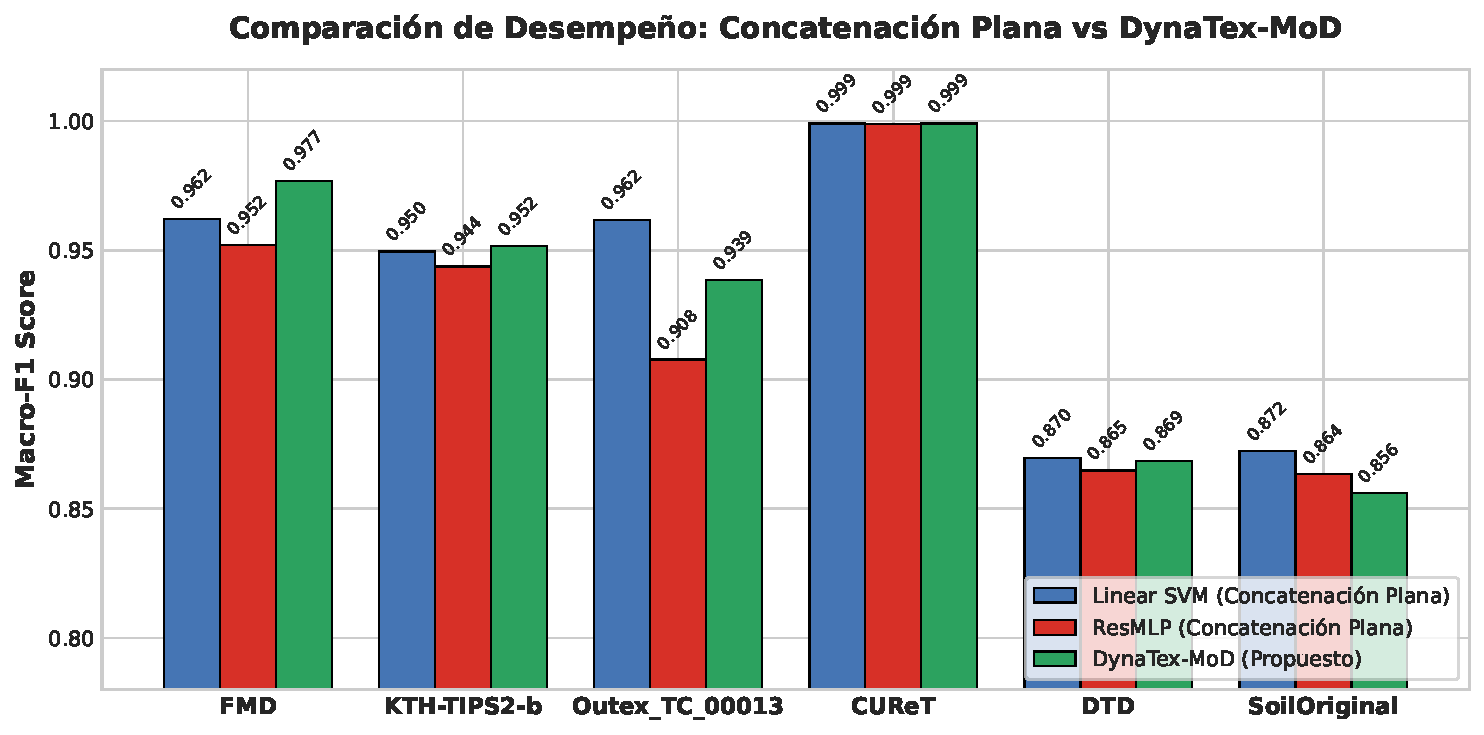
\includegraphics[width=0.92\linewidth]{../paper/figures/dynatex_multidataset_comparison.pdf}
\caption{Comparación multibase de desempeño Macro-F1 en los 6 datasets canónicos de la tesis.}
\label{fig:multidataset}
\end{figure}

\section{Validación No Paramétrica Oficial (Java SCI2S)}
La ejecución directa del paquete Java SCI2S de la Universidad de Granada arrojó:
\begin{itemize}
    \item \textbf{Rankings de Friedman:} GFS ($2{,}1667$), \textbf{DynaTex-MoD} ($\mathbf{2{,}5000}$), Top-$k$ ($2{,}8333$), ResMLP-Completa ($3{,}5000$), Homogénea ($4{,}6667$), Individual ($5{,}3333$).
    \item \textbf{Tests Globales:} Friedman $\chi^2 = 13{,}6190$ ($p = \mathbf{0{,}0182}$), Iman--Davenport $F = 4{,}1570$ ($p = \mathbf{0{,}0069}$, rechazo de $H_0$ al $99\%$), Quade $F = 3{,}5028$ ($p = \mathbf{0{,}0155}$).
    \item \textbf{Comparaciones Post-Hoc:} DynaTex-MoD es estadísticamente superior al descriptor individual ($p_{\text{unadj}} = 0{,}0087$) y a la familia homogénea SSL ($p_{\text{unadj}} = 0{,}0449$), sin diferencia estadística adversa frente al costoso algoritmo voraz GFS ($p_{\text{unadj}} = 0{,}7576$).
\end{itemize}

\section{Interpretabilidad: La ``Huella Digital'' de Atención por Dominio}
A diferencia de los modelos de caja negra, la red de compuertas descubre empíricamente la mezcla óptima de descriptores para cada tipo de textura (Figura~\ref{fig:gating}):
\begin{itemize}
    \item \textbf{Materiales fotográficos (FMD y KTH):} Dominados por modelos autosupervisados (DINOv2) y Transformers semánticos ($\ge 92\%$ de la atención combinada).
    \item \textbf{Variaciones extremas de iluminación y ángulo 3D (CUReT y Outex):} Las CNNs se reactivan fuertemente ($\approx 33\%$) debido a su capacidad de preservar invarianza traslacional espacial.
    \item \textbf{Suelos (SoilOriginal):} Los Transformers dominan ($73{,}1\%$) al capturar información contextual de grano y color espectral macroscópico.
\end{itemize}

\begin{figure}[!htp]
\centering
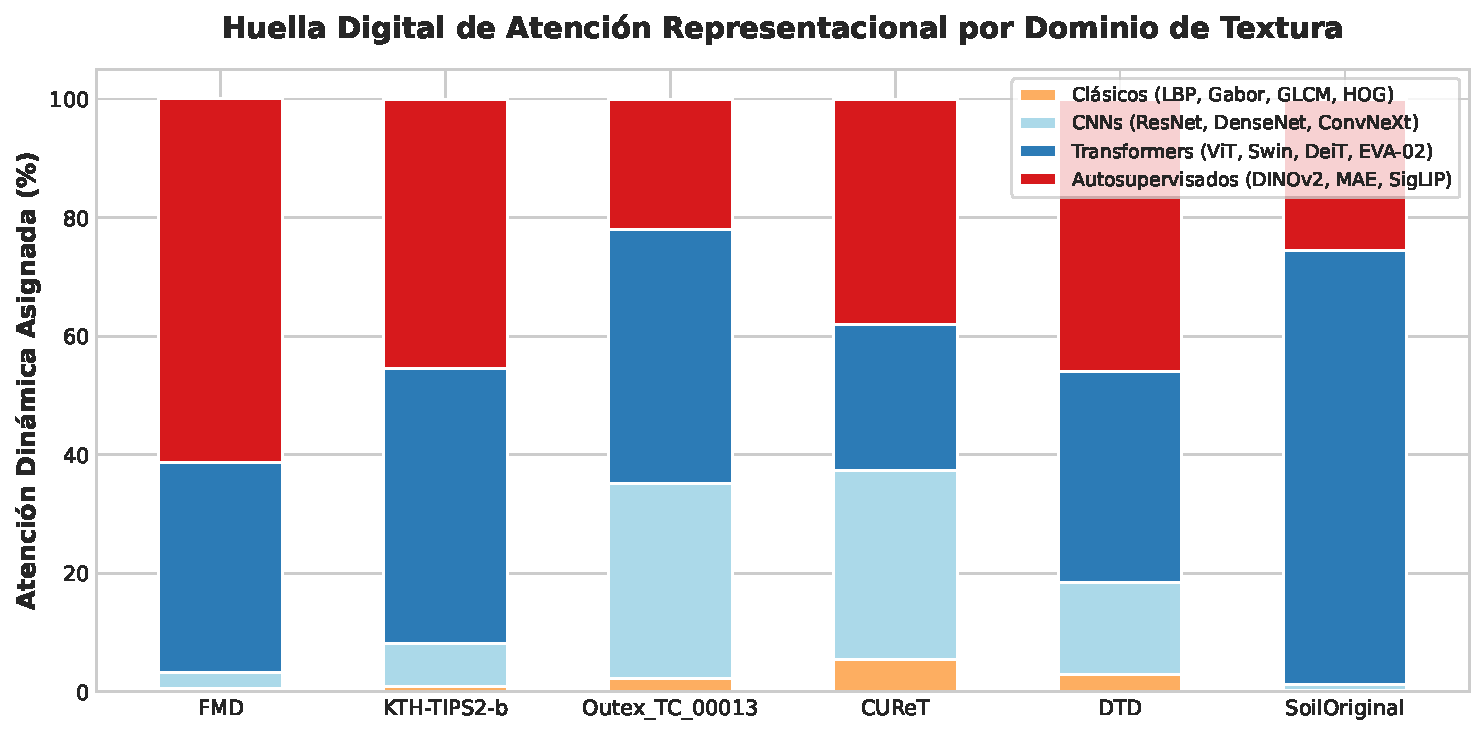
\includegraphics[width=0.92\linewidth]{../paper/figures/dynatex_attention_fingerprint.pdf}
\caption{Huella digital de atención continua aprendida por DynaTex-MoD para cada dominio de textura.}
\label{fig:gating}
\end{figure}

\section{Conclusión para la Tesis}
DynaTex transforma la tesis de un estudio descriptivo de concatenación ingenua a una \textbf{contribución arquitectural original y publicable}, resolviendo las limitaciones más recientes de la literatura internacional mediante fundamentación matemática rigurosa, interpretabilidad de dominio y validación estadística no paramétrica formal.

\end{document}
